\section{Cubic: degree=3}
\label{sec.cubic}

\subsection{Objectives}
The assignment in this section is:
\begin{enumerate}
\item Complete the file \code{src/cubic.py} by writing a Python
  function which computes and returns the x-intercepts of a curve
  equation is \[y=a x^3 + b x^2 + c x + d\,.\]
\item You'll need to replace all occurances of \code{raise NotImplementedError()}
  with correct python code which passes the tests.

\item Complete the file \code{src/search.py} by completing the function \\
  \code{search\_root\_right}
  which follows a similar pattern to that of \\
  \code{search\_root\_left} which you have all the code for.

\item Test the function in GitHub Codespaces by running the file\\
  \code{test/test\_cubic.py}.
\end{enumerate}

\subsection{Overview}


A polynomial of degree 3 has the form $P(x) = a x^3 + b x^2 + c x + d$. If $a=0$ than $P(x)$ is really
a quadratic polynomial (degree 2) and can be solved using the techniques described in Section~\ref{sec.quadratic}.  Every polynomial of degree 3
with real coefficients (for which $a\neq 0$) has at least one real root because 
\begin{enumerate}
\item Either $\lim\limits_{x\to-\infty}P(x) = -\infty$ and $\lim\limits_{x\to\infty}P(x) = \infty$,
  \item Or $\lim\limits_{x\to-\infty}P(x) = \infty$ and $\lim\limits_{x\to\infty}P(x) = -\infty$.
\end{enumerate}


We have a two cubic equations plotted in Figure~\ref{fig.cubic}.

\begin{figure}
  \centering
%% derived from https://tex.stackexchange.com/questions/357538/graph-of-a-parabola-on-pgfplots
%% Thanks to Stefan Pinnow
%%     https://tex.stackexchange.com/users/95441/stefan-pinnow

\begin{figure}
\centering
\begin{tikzpicture}[baseline]
    \begin{axis}[
        width=3in,
        height=3in,
        axis lines=middle,
        xmin=-5,
        xmax=6,
        ymin=-60,
        ymax=60,
%        xtick={20000},
        % ---------------------------------------------------------------------
        % you don't want the ticks/tick labels to be scaled
        scaled ticks=false,
%        % and the tick labels are shown by default the way you want them,
%        % so you don't need to specify them explicitely
%        xticklabels={$20000$},
        % ---------------------------------------------------------------------
 %       ytick={\empty},
        ticklabel style={font=\scriptsize},
        xlabel=$x$,
        ylabel=$y$,
        axis line style={
            latex-latex,
            shorten >=-12.5pt,
            shorten <=-12.5pt,
        },
        xlabel style={at={(ticklabel* cs:1)}, xshift=12.5pt, anchor=north west},
        ylabel style={at={(ticklabel* cs:1)}, yshift=12.5pt, anchor=south west},
    ]

        \addplot[samples=51,smooth,domain=-10:10,color=blue] {x^3 - 4*x^2 - 2*x - 10};

    \end{axis}


\end{tikzpicture}
%
\begin{tikzpicture}[baseline]
    \begin{axis}[
        width=3in,
        height=3in,
        axis lines=middle,
        xmin=-5,
        xmax=6,
        ymin=-60,
        ymax=60,
%        xtick={20000},
        % ---------------------------------------------------------------------
        % you don't want the ticks/tick labels to be scaled
        scaled ticks=false,
%        % and the tick labels are shown by default the way you want them,
%        % so you don't need to specify them explicitely
%        xticklabels={$20000$},
        % ---------------------------------------------------------------------
 %       ytick={\empty},
        ticklabel style={font=\scriptsize},
        xlabel=$x$,
        ylabel=$y$,
        axis line style={
            latex-latex,
            shorten >=-12.5pt,
            shorten <=-12.5pt,
        },
        xlabel style={at={(ticklabel* cs:1)}, xshift=12.5pt, anchor=north west},
        ylabel style={at={(ticklabel* cs:1)}, yshift=12.5pt, anchor=south west},
    ]

        \addplot[samples=51,smooth,domain=-10:10,color=blue] {-x^3 + 4*x^2 + 2*x + 10};

    \end{axis}


\end{tikzpicture}
\caption{Cubics: [left] $y=P_1(x) = x^3 - 4*x^2 - 2*x - 10$,\\[2pt] [right] $y=P_2(x) = -P_1(x) = -x^3 + 4*x^2 + 2*x + 10$}
\label{fig.cubic}
\end{figure}

  %
  \caption{Cubics}
  \label{fig.cubic}
\end{figure}

\begin{align*}
  P_1(x) &= x^3 - 4*x^2 - 2*x - 10\\
  P_2(x) = -P_1(x) &= -x^3 + 4*x^2 + 2*x + 10
\end{align*}

$P_1(x)$ exemplifies the \emph{standard} case where the leading coefficient is positive: $a>0$.
$P_2(x)$ exemplifies the alternate case where the leading coefficient is negative: $a<0$.
However, we notice that $P_1(x)$ and $-P_1(x)$ have the exact same roots, because if $P_2(x) = -P_1(x) = 0$,
then $P_1(x) = 0$.  Therefore, if $a<0$, we can simply find the roots of $-a x^3 -b x^2 - c x - d$;
\ie, we simply negate the coefficients and find the roots of the negated cubic polynomial.


\subsection{Programmatically Computing Roots of a Cubic}

Steps for computing roots of a cubic polynomial.

\begin{enumerate}
\item Assume the coefficients of $P(x) = a x^3 + b x^2 + c x + d$ are
  \code{a},  \code{b},  \code{c},  and~\code{d}.
\item If \code{a==0}, then delegate to the previous solution by
  calling \\
  \code{find\_quadratic\_roots} and returning its return
  value.  Be careful, \code{find\_quadratic\_roots} accepts 3 input
  parameters.
\item If $P(x)$ is of the form of $P_2(x)$ in Figure~\ref{fig.cubic},
  \ie, if $a<0$, then compute and return the roots of $-P(x)$.  To
  compute the roots of $-P(x)$ we simply return
  \code{find\_cubic\_roots(-a, -b, -c, -d)}.
\item Since $P(0) = d$, then we can easily evaluate the polynomial at 0 to get its y-intercept.
  \begin{enumerate}
  \item If $d = 0$, then 0 is a root, $P(0) = 0$.
  \item If $d>0$ then there is a root on the negative x-axis.  Find it with a binary search.
  \item If $d<0$ then there is a root on the positive x-axis. Find it with a binary search.
  \end{enumerate}
\item See Section~\ref{sec.binary.search} to explain the binary search.
\item Once the root $r$ is found, this means $(x-r)$ factors out $P(x)$. \Ie,
  \begin{align*}
    P(x) &= (x-r)(A x^2 + B x + C)\\ 
    A &= a\\
    B &= b + a r \\
    &= b + A r\\
    C &= c + b r + a r^2 \\
    &=
    c + B r\\
  \end{align*}
\item The roots of the cubic are \code{[r]} concatenated to the roots of the quadratic 
  $A x^2 + B x + C$, which you can compute using the techniques in Section~\ref{sec.quadratic}.
\end{enumerate}


\subsection{Find a root using Binary Search}
\label{sec.binary.search}


\begin{figure}
  \centering
%% derived from https://tex.stackexchange.com/questions/357538/graph-of-a-parabola-on-pgfplots
%% Thanks to Stefan Pinnow
%%     https://tex.stackexchange.com/users/95441/stefan-pinnow

  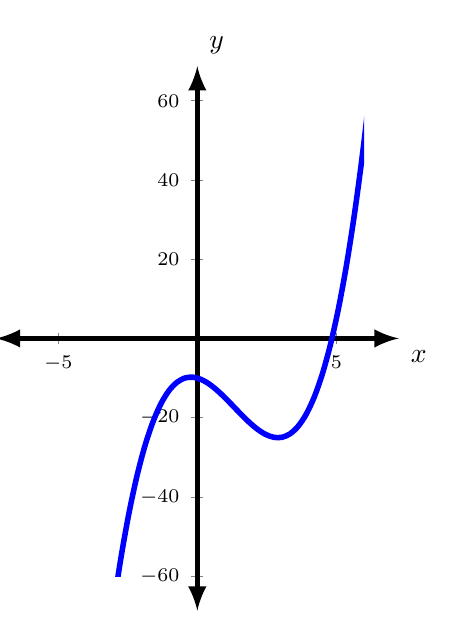
\begin{tikzpicture}[baseline]
    \begin{axis}[
        samples=70,
        smooth,
        domain=-10:10,
        line width=2pt,
        width=0.48\textwidth,
        height=3in,
        axis lines=middle,
        xmin=-6,
        xmax=6,
        ymin=-60,
        ymax=60,
        scaled ticks=false,
        ticklabel style={font=\scriptsize},
        xlabel=$x$,
        ylabel=$y$,
        legend pos=south west,
        legend style={
          anchor=east
        },
        axis line style={
          latex-latex,
          shorten >=-12.5pt,
          shorten <=-12.5pt,
        },
        xlabel style={at={(ticklabel* cs:1)}, xshift=12.5pt, anchor=north west},
        ylabel style={at={(ticklabel* cs:1)}, yshift=12.5pt, anchor=south west},
      ]
      \addplot[color=blue] {x^3 - 4*x^2 - 2*x - 10};
    \end{axis}
  \end{tikzpicture}

  %
  \caption{Expanding Binary Search} 
  \label{fig.cubic.binary}
\end{figure}

Consider the graph of the cubic polynomial shown in Figure~\ref{fig.cubic.binary}.  We'd like to
iteratively find a root; we will use the following steps.

\begin{enumerate}
\item If $P(0)=0$, then we know the root, $x=0$.
\item \label{step.2} If $P(0)< 0$, then find a value of $x_{upper}$ (to the right of 0, $x_{upper}>0$) such that either $P(x_{upper})>0$.
  Now take $x_{lower}=0$.
  Thus we
  will know there is a root in the interval $[x_{lower}, x_{upper}]$.
\item \label{step.3} If $P(0)> 0$, then find a value of $x_{lower}$ (to the left of 0, $x_{lower}<0$) such that either $P(x_{lower})<0$. 
  Now take $x_{upper}=0$.
 Thus we
  will know there is a root in the interval $[x_{lower}, x_{upper}]$.
\item \label{step.4} Since we know there is a root in the interval
  $[x_{lower}, x_{upper}]$, we can divide the interval into two
  intervals.  With the midpoint of the interval, \[x_{mid} =
  \frac{x_{upper} + x_{lower}}{2}\,,\] we consider two intervals:
  $[x_{lower}, x_{mid}]$ and $[x_{mid}, x_{upper}]$.  At least one of
  the following is true:
  \begin{enumerate}
  \item $x_{upper} - x_{right} < \varepsilon$, for some small epsilon (\eg, $\varepsilon = 0.00001$),
    then we know the root is $x_{mid} \pm \varepsilon$, which is good enough.
  \item $P(x_{mid}) = 0$, then we know the root $x= x_{mid}$.
  \item There is a root in the interval $[x_{lower}, x_{mid}]$, then
    we repeat step~\ref{step.4} on the intveral $[x_{lower},
      x_{mid}]$.
  \item There is a root in the interval $[x_{mid}, x_{upper}]$, then
    we repeat step~\ref{step.4} on the interval $[x_{mid},
      x_{upper}]$.
  \end{enumerate}
\end{enumerate}


How does step~\ref{step.2} work?  Start with  $x_{upper}=1$, and query whether ${P(x_{upper}) < 0}$.
If so, then double $x_{upper}$ and try again, until ${P(x_{upper}) > 0}$.  As an example with the polynomial in Figure~\ref{fig.cubic.binary}, we would try ${P(1)< 0}$, ${P(2) < 0}$, ${P(4)<0}$, and finally ${P(8) > 0}$.

Similarly for step~\ref{step.3}?  Start with  $x_{upper}=-1$, and query whether ${P(x_{lower}) > 0}$.
If so, then double $x_{upper}$ and try again, until ${P(x_{upper}) < 0}$.
